\documentclass{article}
%Packages
\usepackage{graphicx} % Required for inserting images
\usepackage{titling} % per l'uso di \theauthor, \thetitle
\usepackage[a4paper, margin=2cm]{geometry}
% === per indice
\usepackage{makeidx}
\usepackage{tocloft}
%====
\usepackage{fancyhdr} % per il layout di intestazione e piè di pagina
\usepackage{tcolorbox} % per le box colorate
\usepackage{float} % per il posizionamento delle immagini
\usepackage{caption} % per impostare figura invece di figure
\usepackage[hidelinks]{hyperref} % per \nameref e hyperlink ai riferimenti
% ==== matematica
\usepackage{amsmath}
\usepackage{amssymb}
% === snippet di codice ==== %
\usepackage{minted}
\usepackage[svgnames]{xcolor}
% ========================== %
\usepackage{subfigure}  % allineare le immagini comodamente
%Package per tabella test
\usepackage{booktabs}
\usepackage{longtable}
\usepackage{xcolor}
\usepackage{geometry}
% Titolo bibliografia in italiano
\renewcommand{\refname}{Bibliografia}
% Percorso delle immagini 
\graphicspath{{./images/}}

\title{Relazione Ingegneria del software}
\author{Salvatore Greco, Stefano Marianelli}

\captionsetup[figure] {name=Figura} 
\captionsetup[table] {name=Tabella} 
\captionsetup[listing] {name=Codice} 
%Impostazioni dell'indice
\renewcommand{\cftsecleader}{\cftdotfill{\cftdotsep}} % per avere i puntini fra titolo del paragrafo e numero di pagina
\setlength{\cftbeforesecskip}{8pt} 
\renewcommand{\contentsname}{Indice} % Titolo dell'indice
% ================ %
\begin{document}
% Frontespizio
\begin{titlepage}
\begin{figure}[H]
    \centering
    \includegraphics[width=\linewidth]{images/logo_unifi.png}
    \label{fig:logo_unifi}
\end{figure}
\vspace{1cm}
%{\centering \includegraphics[width=\textwidth]{logo_unifi} \par} 

{\centering \huge {\textbf{\thetitle}}\par} \vspace{2cm}

{\large 
\textit{Candidati:} \theauthor \hfill
\textit{Corso:} Ingegneria del Software \\ 


\textit{Anno Accademico: } 2025/2026 \hfill
\textit{Docente:} Prof. Enrico Vicario
}
\end{titlepage}

%Indice
\tableofcontents
\newpage
%Capitolo 1
\section{Introduzione}
Il presente elaborato è stato scritto per il superamento dell'esame Ingegneria Del Software del corso di laurea triennale in Ingegneria Informatica dell'Università degli Studi di Firenze.\newline
Si descrive il design e l'implementazione in \textit{Java} di un sistema gestionale per biblioteche. \newline

Il progetto è stato versionato usando Git e l'intero codice sorgente è disponibile all'url \url{https://github.com/salvatore-greco/SWE}. Sono state usate due GitHub Action per gestire il deploy su GitHub Pages dei risultati di coverage e per la compilazione della presente relazione.


\subsection{Statement}
Il progetto modella un sistema di gestione per biblioteche comunali, prendendo d'ispirazione le biblioteche del comune di Firenze.
Il sistema permette la gestione da parte del personale della biblioteca del proprio catalogo di libri permettendone l'aggiunta, la modifica e la cancellazione. Semplifica le operazioni di prestito permettendo agli utenti di prenotare una copia da prendere successivamente in biblioteca; essa deve essere approvata dal bibliotecario per registrarne l'effettivo prestito; inoltre può essere effettuato anche senza prenotazione, recandosi in biblioteca e registrandone il prestito dal bibliotecario. Permette inoltre di gestire eventi, come mostre di libri, incontri con gli autori, mostrando dettagli sulla data, luogo e durata dell'evento e permettendo agli utenti di riservare un posto nell'aula. 
I servizi offerti sono disponibili attraverso la richiesta della tessera della biblioteca. L'utente sprovvisto di tessera, ma provvisto di credenziali può farne richiesta, presentandosi poi in biblioteca per il suo rilascio fisico tramite il bibliotecario.
L'amministratore della biblioteca può gestirne il budget e il catalogo attraverso le operazioni CRUD sui libri descritte precedentemente.
Se provviste di aule studio, ne permette la gestione: consultare i posti disponibili  e prenotarne uno; essi vengono rilasciati in modo automatico giornalmente e possono essere rilasciati manualmente da parte degli utenti.    

\subsection{Architettura e tecnologie utilizzate}\label{subsec:architettura}
Per lo sviluppo è stato utilizzato \textit{Java}, utilizzando come IDE \textit{IntelliJ} data la sua grande integrazione con l'ecosistema e col database.
Come database è stato scelto \textit{PostgreSQL}, utilizzando le API \textit{JDBC} e il suo relativo driver. Use Case Diagram e Class Diagram seguono lo standard UML e sono stati realizzati col software \textit{StarUML}.\newline
Sono state usate le seguenti dipendenze esterne, gestite attraverso il build system \textit{Maven}:
\begin{itemize}
    \item \textbf{PostgreSQL JDBC driver}
    \item \href{https://github.com/cdimascio/dotenv-java}{\textbf{dotenv-java}}: per la gestione delle variabili d'ambiente in file \textit{.env} per il collegamento al database
    \item \textbf{spring-security-crypto}: per l'hashing delle password attraverso l'algoritmo \textit{Bcrypt}
    \item \textbf{JUnit}
    \item \textbf{spring-jdbc}: per l'esecuzione di script da file \textit{.sql}. Usato per l'inizializzazione e la pulizia del database nello schema test.
    \item \textbf{Mockito}: per la creazione di mock e stub per Unit Testing.
    \item \textbf{JaCoCo}: per statistiche di copertura dei test.
\end{itemize}
Il progetto è stato diviso in quattro package: DomainModel, BusinessLogic, ORM, Exception.\newline
Per la business logic è stato scelto di creare un controller per attore data l'assenza di una GUI. Data questa circostanza è stato scritto un ampio numero di test case, fra Unit Test e Integration Test.
\begin{figure}[H]
    \centering
    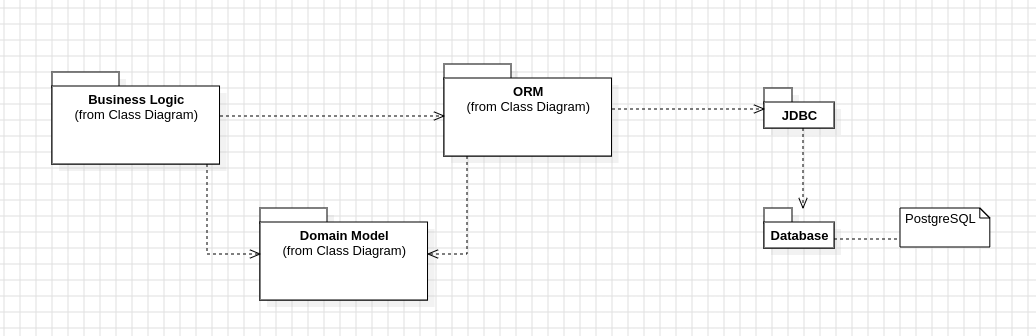
\includegraphics[width=1\linewidth]{images/package_diagram.png}
    \caption{Package diagram del progetto}
    \label{fig:placeholder}
\end{figure}
%Capitolo 2
\section{Progettazione}

\subsection{Use Case Template}
Di seguito vengono descritti i template per i casi d'uso indicati nello Use Case Diagram.
\subsubsection{Login}
\begin{table}[h!]
    \begin{tabularx}{\textwidth}{|c|X|}
    \hline
        \textbf{Use Case Template} \#1 & Login  \\ \hline
        \textbf{Descrizione} & L'utente accede al sistema attraverso le proprie credenziali \\ \hline
        \textbf{Livello} & User Goal \\ \hline
        \textbf{Attori} & Library User, Librarian o Library Administrator \\ \hline 
        \textbf{Pre Condizioni} & L'utente è nella pagina appropriata e non ha già fatto il login \\ \hline
        \textbf{Basic Flow} & \begin{enumerate}[nosep, leftmargin=* ,before=\vspace{-0.5\baselineskip}]
            \item L'utente inserisce il nome utente e password 
            \item L'utente invia le credenziali 
            \item Il sistema controlla le credenziali 
            \item Il sistema autentica l'utente, istanziandone il proprio controller 
        \end{enumerate} \\ \hline
        \textbf{Alternative Flow} & 3a. Se le credenziali sono errate il sistema restituisce un errore permettendo di ritentare  \\ \hline
        \textbf{Post Condizioni} & L'utente è autenticato. Viene istanziato il controller appropriato\\ \hline
        \textbf{Test} & 1,2,3 \\ \hline
    \end{tabularx}
    \caption{Login UCT}
    \label{tab:Login UCT}
\end{table}

\subsubsection{Registrazione}
\begin{table}[h!]
    \begin{tabularx}{\textwidth}{|c|X|}
    \hline
        \textbf{Use Case Template} \#1 & Registrazione  \\ \hline
        \textbf{Descrizione} & L'utente sprovvisto di credenziali si registra \\ \hline
        \textbf{Livello} & User Goal \\ \hline
        \textbf{Attori} & Library User, Librarian o Library Administrator \\ \hline 
        \textbf{Pre Condizioni} & L'utente è nella pagina appropriata e non ha fatto il login \\ \hline
        \textbf{Basic Flow} & \begin{enumerate}[nosep, leftmargin=* ,before=\vspace{-0.5\baselineskip}]
            \item L'utente inserisce nome, cognome, email, password 
            \item L'utente invia le credenziali 
            \item Il sistema controlla che non esista già un utente con l'email inserita 
            \item Il sistema crea l'account 
        \end{enumerate} \\ \hline
        \textbf{Alternative Flow} & 3a. Se l'utente esiste già restituisce un errore permettendo di ritentare  \\ \hline
        \textbf{Post Condizioni} & Viene creato l'account, permettendo all'utente di fare il login\\ \hline
        \textbf{Test} & 1,2,3 \\ \hline
    \end{tabularx}
    \caption{Registrazione UCT}
    \label{tab:Registrazione UCT}
\end{table}

\subsubsection{Reset password}
\begin{table}[H]
    \begin{tabularx}{\textwidth}{|c|X|}
    \hline
        \textbf{Use Case Template} \#1 & Reset password  \\ \hline
        \textbf{Descrizione} & Permette all'utente che si è dimenticato la propria password di recuperare il profilo reimpostando la password \\ \hline
        \textbf{Livello} & User Goal \\ \hline
        \textbf{Attori} & Library User, Librarian o Library Administrator \\ \hline 
        \textbf{Pre Condizioni} & L'utente è nella pagina appropriata, dopo aver ricevuto la possibiltà di recuperare la password confermando la propria identità \\ \hline
        \textbf{Basic Flow} & \begin{enumerate}[nosep, leftmargin=* ,before=\vspace{-0.5\baselineskip}]
            \item L'utente inserisce la nuova password, confermandola 
            \item L'utente invia le credenziali 
            \item Il sistema cambia la password con quella indicata 
        \end{enumerate} \\ \hline
        \textbf{Alternative Flow} & -  \\ \hline
        \textbf{Post Condizioni} & Viene resettata la password\\ \hline
        \textbf{Test} & 1,2,3 \\ \hline
    \end{tabularx}
    \caption{Reset password UCT}
    \label{tab:Reset password UCT}
\end{table}
%Capitolo 3
\section{Implementazione}
In questa sezione vengono descritte le principali classi e interfacce implementate, organizzate nei rispettivi package in base al loro ruolo all'interno del sistema.

\subsection{Domain Model}
Il Domain Model, mostrato in Figura~\ref{fig:domain_model}, rappresenta l'insieme delle entità fondamentali del dominio applicativo e le relazioni tra di esse. 
Ogni classe modella un concetto reale presente nel sistema di gestione della biblioteca.
\begin{figure}[H]
    \centering
    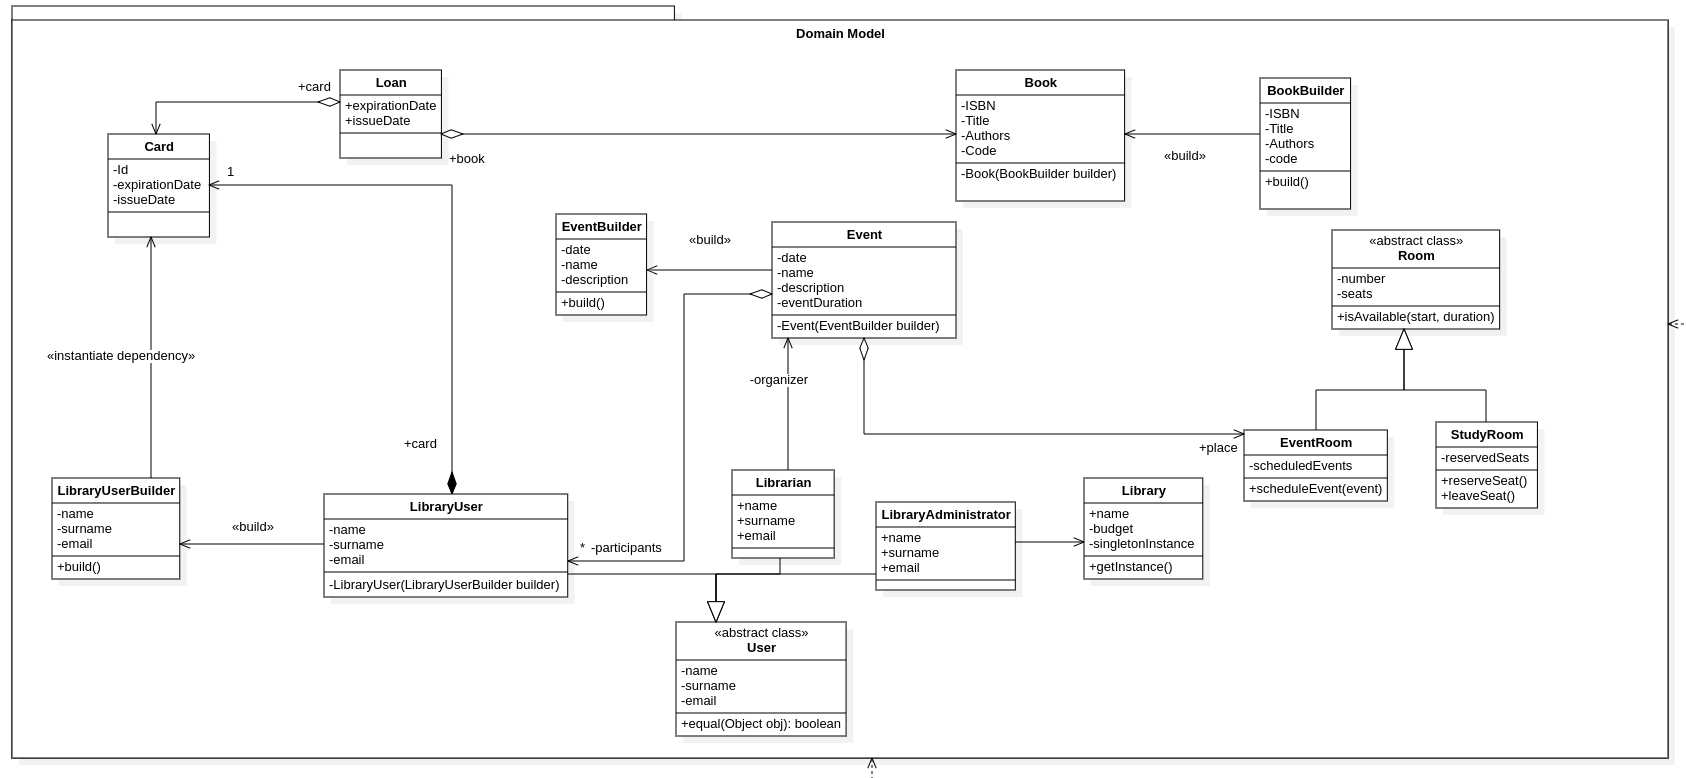
\includegraphics[width=\linewidth]{images/class diagram/domain_model.png}
    \caption{Domain Model del sistema}
    \label{fig:domain_model}
\end{figure}

    \subsubsection{Library}
    Questa classe rappresenta la biblioteca. È caratterizzata da un nome ed un budget che ha a disposizione.\\
    Per l'istanza di una Library viene utilizzato il design pattern del \textbf{singleton}, in modo tale da avere un unica istanza in tutto il sistema.
    
    \subsubsection{Book}
    Questa classe rappresenta un libro.\\
    Questo può essere aggiunto o rimosso dal catalogo di tutti i libri della biblioteca da parte dell'amministratore della biblioteca. Se presente nel catalogo, può essere preso in prestito da un utente ed è identificato tramite ISBN, titolo e codice. Inoltre su questo è riportato anche il nome degli autori.\\
    Per la creazione di un oggetto Book viene usato il \textbf{BookBuilder}, che implementa il design pattern del \textbf{builder}.\\

    \subsubsection{Loan}
    Questa classe rappresenta un prestito di un libro da parte di un utente.\\

    \subsubsection{User}
    Questa classe rappresenta un utente astratto, caratterizzato da nome, cognome ed email. La classe appunto è definita come astratta.\\

     \subsubsection{LibraryUser}
    Questa classe rappresenta un utente che può usufruire i servizi messi a disposizione dalla biblioteca, come il prestito di libri, l'iscrizione ad eventi o la prenotazione posti nelle aule studio.\\
    La creazione degli oggetti avviene tramite il design pattern \textbf{Builder}.
    
    \subsubsection{Librarian}
    Questa classe rappresenta un bibliotecario, un utente con permessi aggiuntivi, che lavora all'interno della biblioteca. Può gestire gli eventi, creare/rinnovare tessere della biblioteca e monitorare i prestiti.\\
    
    \subsubsection{LibraryAdministrator}
    Questa classe rappresenta l'amministratore della biblioteca.\\
    Oltre alla gestione del catalogo libri, è anche responsabile dei fondi della biblioteca.
    
    \subsubsection{Card}
    Questa classe rappresenta una tessera della biblioteca associata a un utente.\\
    La tessera consente l'accesso ai servizi della biblioteca, come il prestito di libri e la prenotazione di risorse ed è identificata tramite id, data di emissione e scadenza della carta.\\
    
    \subsubsection{Event}
    Questa classe rappresenta un evento organizzato dalla biblioteca.\\
    È identificato tramite un id univoco e caratterizzato da nome, descrizione, data, durata e luogo.\\
    La creazione degli oggetti avviene tramite l'\textbf{EventBuilder}, che implementa il design pattern \textbf{Builder}.\\

    \subsubsection{Room}
    Questa classe rappresenta una stanza generica della biblioteca.\\
    È identificata tramite un numero, la sua capacità e un attributo che indica se si tratta di un aula studio.\\
    
    \subsubsection{EventRoom}
    Questa classe rappresenta una stanza che può essere adibita allo svolgimento di eventi.\\
    
    \subsubsection{StudyRoom}
    Questa classe rappresenta una stanza dedicata esclusivamente per lo studio.\\
    


\subsection{Business Logic}
La Business Logic, mostrata in Figura~\ref{fig:business_logic}, contiene tutte le classi responsabili della gestione delle funzionalità del sistema e dell'interazione tra le diverse entità del Domain Model.
\begin{figure}[H]
    \centering
    
\includegraphics[width=\linewidth]{images/class diagram/business_logic.png}
    \caption{Business Logic del sistema}
    \label{fig:business_logic}
\end{figure}

    \subsubsection{AuthService e ConcreteAuthService}
    L'\texttt{AuthService} è un'interfaccia che dichiara i principali metodi di autenticazione: \textbf{login, logout, register e resetPassword,}.\\
    Questi vengono implementati in \texttt{ConcreteAuthService}. In particolare, il metodo \textbf{login} restituisce un tipo di utente diverso in base al ruolo dell'utente autenticato.\\
    La gestione della sessione di un utente, è realizzato tramite il metodo \textbf{isLogged}, che verifica se un utente è autenticato o meno.\\

    \subsubsection{role}
    Il \texttt{role} è un \textbf{enum} che identifica i possibili ruoli degli utenti del sistema: \textbf{LibraryUser, Librarian e LibraryAdministrator}.\\

    \subsubsection{ControllerInterface}
    La \texttt{ControllerInterface} è un'interfaccia di supporto, che dichiara il metodo \textbf{createController}, il quale restituisce un oggetto di tipo \texttt{ControllerInterface}.\\
    Questa interfaccia implementa il design pattern \textbf{Factory}, consentendo la creazione dei diversi controller in base al tipo di utente.

    \subsubsection{ControllerFactory}
    La \texttt{ControllerFactory} è un'interfaccia che dichiara il metodo \textbf{createController}, il quale restituisce un oggetto di tipo \texttt{ControllerInterface}.\\
    Questa interfaccia implementa il design pattern \textbf{Factory}, consentendo la creazione dei diversi controller in base al tipo di utente.

    \subsubsection{LibraryUserControllerFactory}
    Questa classe implementa l'interfaccia \texttt{ControllerFactory} e sovrascrive il metodo \textbf{createController}, restituendo un'istanza di \texttt{LibraryUserController}.

    \subsubsection{LibraryUserController}
    La classe \texttt{LibraryUserController} definisce un interfaccia per gli utenti della biblioteca che come anticipato possono:
    \begin{itemize}
        \item richiedere in prestito un libro con \textbf{requestLoan}, se l'utente possiede una carta non scaduta e se il libro è disponibile nel catalogo. 
        \item richiedere una tessera della biblioteca con \textbf{requestCard}, se l'utente non nè possiede già una.
        \item prenotare un posto in un aula studio con \textbf{reserveSeatStudyRoom}, se l'utente non ha già effettuato una prenotazione e se la stanza non è piena.
        \item lasciare un posto in un aula studio con \textbf{leaveSeatStudyRoom}.
        \item prenotare un posto ad un evento con \textbf{eventBooking}.
        \item cancellare una prenotazione ad un evento con \textbf{cancelEventBooking}.
    \end{itemize}

    \subsubsection{LibrarianControllerFactory}
    Questa classe implementa l'interfaccia \texttt{ControllerFactory} e sovrascrive il metodo \textbf{createController}, restituendo un'istanza di \texttt{LibrarianController}.

    \subsubsection{LibrarianController}
    La classe \texttt{LibrarianController} definisce invece tutte le operazioni per i bibliotecari, che sono:
    \begin{itemize}
        \item creare o rinnovare una tessera con \textbf{createCard}.
        \item creare un evento con \textbf{createEvent}.
        \item cancellare un evento con \textbf{cancelEvent}.
        \item modificare un evento con \textbf{modifyEvent}.
        \item registrare un prestito con \textbf{registerLoan}.
        \item rinnovare un prestito con \textbf{grantLoan}.
        \item terminare un prestito con \textbf{endLoan}.
    \end{itemize}

    \subsubsection{LibraryAdministratorControllerFactory}
    Questa classe implementa l'interfaccia \texttt{ControllerFactory} e sovrascrive il metodo \textbf{createController}, restituendo un'istanza di \texttt{LibraryAdministratorController}.

    \subsubsection{LibraryAdministratorController}
    La classe \texttt{LibraryAdministratorController} infine definisce tutte le operazioni disponibili per l'amministratore della biblioteca, che sono:
    \begin{itemize}
        \item aumentare il budget della biblioteca con \textbf{increaseBudget}, il quale non può essere negativo.
        \item aggiungere un libro al catalogo con \textbf{addBookToCatalogue}.
        \item rimuovere un libro dal catalogo con \textbf{removeBookFromCatalogue}.
        \item aggiornare un libro nel catalogo con \textbf{updateBookInCatalogue}.
    \end{itemize}

\subsection{ORM}
%Capitolo 4
\section{Testing}
I test sono stati eseguiti tramite il framework \texttt{JUnit} e sono stati strutturati come segue:
\begin{verbatim}
 src/test/
`-- java
    |-- IntegrationTest
    |   |-- BookIntegrationTest.java
    |   |-- CardIntegrationTest.java
    |   |-- EventIntegrationTest.java
    |   |-- LibraryIntegrationTest.java
    |   |-- LoanIntegrationTest.java
    |   |-- ORM
    |   |   |-- BaseIntegrationTest.java
    |   |   |-- BookDAOIntegrationTest.java
    |   |   |-- CardDAOIntegrationTest.java
    |   |   |-- ConnectionManagerUnitTest.java
    |   |   |-- EventDAOIntegrationTest.java
    |   |   |-- LibraryDAOIntegrationTest.java
    |   |   |-- LoanDAOIntegrationTest.java
    |   |   |-- RoomDAOIntegrationTest.java
    |   |   `-- UserDAOIntegrationTest.java
    |   `-- StudyRoomIntegrationTest.java
    `-- UnitTest
        |-- BusinessLogic
        |   `-- AuthUnitTest.java
        |-- DomainModel
        |   |-- EventRoomUnitTest.java
        |   |-- EventUnitTest.java
        |   |-- LoanUnitTest.java
        |   |-- RoomUnitTest.java
        |   `-- StudyRoomUnitTest.java
        `-- utils
            |-- DBSeeder.java
            `-- DBSeederTest.java
\end{verbatim}
Sono stati divisi nei package \texttt{UnitTest} e \texttt{IntegrationTest}. Nel primo si va a testare la classe in isolamento, facendo il mock del database se necessario, come fatto un \texttt{AuthUnitTest} di cui si riporta un estratto di codice; mentre nel secondo si vanno a chiamare i metodi implementati nei DAO interrogando realmente il database. Per l'elenco di tutti i test case si rimanda alla sezione \hyperref[tabella_test]{Tabella test}.
\begin{code}
\begin{minted}{java}
@BeforeAll
    public static void init() {
        userDAO = mock(UserDAO.class);
        when(userDAO.getUserByEmail("library.user@email.com")).thenReturn(new UserDTO(
                "library.user@email.com",
                "Mario",
                "Rossi",
                role.libraryUser,
                BCrypt.hashpw("password", BCrypt.gensalt())
        ));
        when(userDAO.getUserByEmail("librarian@email.com")).thenReturn(new UserDTO(
                "librarian@email.com",
                "Luca",
                "Bianchi",
                role.librarian,
                BCrypt.hashpw("bibliotecario", BCrypt.gensalt())
        ));
        when(userDAO.getUserByEmail("admin@email.com")).thenReturn(new UserDTO(
                "admin@email.com",
                "Sara",
                "Verdi",
                role.libraryAdministrator,
                BCrypt.hashpw("admin", BCrypt.gensalt())
        ));
        when(userDAO.getUserByEmail("inesistente@email.com")).thenThrow(new UserNotFoundException("Wrong username or password"));
        when(userDAO.updatePassword(eq("library.user@email.com"), anyString())).thenReturn(true);
        when(userDAO.updatePassword(eq("inesistente@email.com"), anyString())).thenReturn(false);
        when(userDAO.insertUser(any())).thenReturn(false);
        when(userDAO.insertUser(refEq(new UserDTO(
                "nuovo@email.com",
                "Gino",
                "Neri",
                role.libraryUser,
                "password"
        )))).thenReturn(true);
    }
    
    @Test
    public void login_invalidPassword_throwsException() {
        AuthService authService = new ConcreteAuthService(userDAO);
        var e = assertThrows(UserNotFoundException.class, () -> authService.login("library.user@email.com", "Password"));
        assertEquals("Wrong username or password", e.getMessage());
    }
\end{minted}
\caption{init e test case in AuthUnitTest}
\end{code}
\noindent Per agevolare l'automatizzazione degli integration test è stata scritta una classe \texttt{DBSeeder} che va a creare uno schema \texttt{test}, istanziato mediante il file \texttt{db.sql} e popolato tramite il file \texttt{data.sql}. Gli script \textit{SQL} sono eseguiti tramite la classe \texttt{ResourceDatabasePopulator} del package \texttt{springframework.jdbc}
\begin{code}
    \begin{minted}{java}
    public class DBSeeder {

    private Connection connection;

    public DBSeeder() throws SQLException{
        this.connection = ConnectionManager.getInstance().getConnection();
    }

    public void createTestSchema() {
        try {
            Statement stmt = connection.createStatement();
            stmt.executeUpdate("CREATE SCHEMA IF NOT EXISTS test AUTHORIZATION CURRENT_USER");
        } catch (SQLException e) {
            e.printStackTrace();
        }
    }
    public void deleteTestSchema(){
        try {
            connection.setAutoCommit(true);
            Statement stmt = connection.createStatement();
            stmt.executeUpdate("DROP SCHEMA IF EXISTS test CASCADE");
            stmt.executeUpdate("SET search_path TO public");
        } catch (SQLException e) {
            e.printStackTrace();
        }
    }

    public void initDatabaseTest(String filenameDDL, String filenameData){
        try {
            Statement stmt = connection.createStatement();
            stmt.execute("SET search_path TO test");
        } catch (SQLException e) {
            e.printStackTrace();
            throw new RuntimeException("Database error. Check if schema 'test' exists");
        }
        ResourceDatabasePopulator populator = new ResourceDatabasePopulator();
        populator.addScripts(
                new FileSystemResource(filenameDDL), //file must be in root directory
                new FileSystemResource(filenameData)
        );
        populator.populate(this.connection);
    }
}
    \end{minted}
\caption{Classe DBSeeder}
\end{code}
\noindent Il setup e il teardown sono comuni a tutti gli integration test; essi sono definiti nella classe \texttt{BaseIntegrationTest} che ogni classe nel package estende. Il setup va a creare lo schema \texttt{test}, crea le tabelle e imposta l'autocommit della connessione a falso; dopo ogni test case viene eseguito il teardown, dove viene fatto il rollback della transazione. In caso di fallimento di questa operazione, viene impostato un flag \texttt{teardownFail} a vero, che il metodo \texttt{teardownChecker} eseguito dopo ogni test case controlla, facendo fallire tutti i test dato lo stato inconsistente del database. Infine il metodo \texttt{connectionCloser} cancella lo schema precedentemente creato e chiude la connessione.
\begin{code}
    \begin{minted}{java}
    private static void setTestSchema() throws SQLException {
        Statement stmt = connDAO.createStatement();
        stmt.execute("SET search_path TO test");
    }

    @BeforeAll
    public static void init() {
        try {
            dbSeeder = new DBSeeder();
        } catch (SQLException e) {
            e.printStackTrace();
            fail("Failed to instantiate DBSeeder. Check connection to db");
        }
        dbSeeder.createTestSchema();
        assertDoesNotThrow(() -> dbSeeder.initDatabaseTest("db.sql", "data.sql"));
        try {
            connDAO = ConnectionManager.getInstance().getConnection();
            setTestSchema();
            connDAO.setAutoCommit(false);
        } catch (SQLException e) {
            e.printStackTrace();
            fail("Fail to get connection");
        }
    }

    @AfterEach
    public void teardown() {
        try {
            connDAO.rollback();
        } catch (SQLException e) {
            teardownFail = true;
            e.printStackTrace();
        }
    }

    @BeforeEach
    public void teardownChecker() {
        assumeFalse(teardownFail, "Aborting test. DB state is inconsistent");
    }


    @AfterAll
    public static void connectionCloser(){
        try {
            dbSeeder.deleteTestSchema();
            connDAO.close();
        } catch (SQLException e) {
            e.printStackTrace();
        }
    }        
    \end{minted}
    \caption{metodi della classe BaseIntegrationTest}
\end{code}
\subsection{Test coverage}
I risultati di copertura sono stati generati con \texttt{JaCoCo} e sono disponibili per la consultazione su \url{https://salvatore-greco.github.io/SWE/}.\\
È stato raggiunto un buon risultato col \textbf{90\%} di linee di codice coperte e il \textbf{79\%} di branch coperti. Il risultato più basso coi branch è causato da alcune condizioni non testate sui ResultSet nei DAO.

\subsection{Unit Test}
In questo package sono presenti gli unit test di alcune classi del package \texttt{DomainModel}, che implementano metodi effettivamente da testare, di \texttt{ConcreteAuthService} del package \texttt{BusinessLogic} e della classe \texttt{DBSeeder}.


%tabella test
% Generato automaticamente da java_to_latex.py
% Sorgente : test
% Data     : 2026-03-27 19:50
% Classi   : 23  |  Metodi totali: 234
\section*{Tabella test}\label{tabella_test}

\subsection*{Business Login Integration test}\label{BL_IT}
\subsubsection*{Classe \texttt{BookIntegrationTest}}
{\small\textit{java/IntegrationTest/BookIntegrationTest.java}}
\vspace{4pt}

\begin{longtable}{@{}llll@{}}
\toprule
\textbf{Visibilita} & \textbf{Modificatori} & \textbf{Tipo ritorno} & \textbf{Nome metodo} \\
\midrule
\endfirsthead
\multicolumn{4}{c}{\small\itshape (continua dalla pagina precedente)} \\
\toprule
\textbf{Visibilita} & \textbf{Modificatori} & \textbf{Tipo ritorno} & \textbf{Nome metodo} \\
\midrule
\endhead
\midrule
\multicolumn{4}{r}{\small\itshape (continua nella pagina seguente)} \\
\endfoot
\bottomrule
\endlastfoot
  public & - & \texttt{void} & \texttt{addBookToCatalogue} \\
  public & - & \texttt{void} & \texttt{addBookToCatalogue\_duplicateBook\_throws} \\
  public & - & \texttt{void} & \texttt{removeBookFromCatalogue} \\
  public & - & \texttt{void} & \texttt{removeBookFromCatalogue\_bookNotAdded\_throws} \\
  public & - & \texttt{void} & \texttt{updateBookInCatalogue} \\
  public & - & \texttt{void} & \texttt{updateBookInCatalogue\_notExistingBook} \\
\end{longtable}

\subsubsection*{Classe \texttt{CardIntegrationTest}}
{\small\textit{java/IntegrationTest/CardIntegrationTest.java}}
\vspace{4pt}

\begin{longtable}{@{}llll@{}}
\toprule
\textbf{Visibilita} & \textbf{Modificatori} & \textbf{Tipo ritorno} & \textbf{Nome metodo} \\
\midrule
\endfirsthead
\multicolumn{4}{c}{\small\itshape (continua dalla pagina precedente)} \\
\toprule
\textbf{Visibilita} & \textbf{Modificatori} & \textbf{Tipo ritorno} & \textbf{Nome metodo} \\
\midrule
\endhead
\midrule
\multicolumn{4}{r}{\small\itshape (continua nella pagina seguente)} \\
\endfoot
\bottomrule
\endlastfoot
  public & - & \texttt{void} & \texttt{createRequestedCard} \\
  public & - & \texttt{void} & \texttt{createCard} \\
  public & - & \texttt{void} & \texttt{requestCard\_userWithCard\_throws} \\
  public & - & \texttt{void} & \texttt{createCard\_userWithCard\_throws} \\
\end{longtable}

\subsubsection*{Classe \texttt{EventIntegrationTest}}
{\small\textit{java/IntegrationTest/EventIntegrationTest.java}}
\vspace{4pt}

\begin{longtable}{@{}llll@{}}
\toprule
\textbf{Visibilita} & \textbf{Modificatori} & \textbf{Tipo ritorno} & \textbf{Nome metodo} \\
\midrule
\endfirsthead
\multicolumn{4}{c}{\small\itshape (continua dalla pagina precedente)} \\
\toprule
\textbf{Visibilita} & \textbf{Modificatori} & \textbf{Tipo ritorno} & \textbf{Nome metodo} \\
\midrule
\endhead
\midrule
\multicolumn{4}{r}{\small\itshape (continua nella pagina seguente)} \\
\endfoot
\bottomrule
\endlastfoot
  public & - & \texttt{void} & \texttt{createEvent} \\
  public & - & \texttt{void} & \texttt{createEvent\_invalidRoom\_throws} \\
  public & - & \texttt{void} & \texttt{createEvent\_pastDate\_throws} \\
  public & - & \texttt{void} & \texttt{createEvent\_negativeDuration\_throws} \\
  public & - & \texttt{void} & \texttt{createEvent\_StudyRoom\_throws} \\
  public & - & \texttt{void} & \texttt{cancelEvent} \\
  public & - & \texttt{void} & \texttt{cancelEvent\_notExisting\_throws} \\
  public & - & \texttt{void} & \texttt{modifyEvent} \\
  public & - & \texttt{void} & \texttt{modifyEvent\_notExisting\_throws} \\
  public & - & \texttt{void} & \texttt{eventBooking} \\
  public & - & \texttt{void} & \texttt{eventBooking\_notExistingEvent\_throws} \\
  public & - & \texttt{void} & \texttt{eventBooking\_alreadyBooked\_throws} \\
  public & - & \texttt{void} & \texttt{cancelEventBooking} \\
  public & - & \texttt{void} & \texttt{cancelEventBooking\_notExistingEvent\_throws} \\
  public & - & \texttt{void} & \texttt{cancelEventBooking\_notBooked\_throws} \\
\end{longtable}

\subsubsection*{Classe \texttt{LibraryIntegrationTest}}
{\small\textit{java/IntegrationTest/LibraryIntegrationTest.java}}
\vspace{4pt}

\begin{longtable}{@{}llll@{}}
\toprule
\textbf{Visibilita} & \textbf{Modificatori} & \textbf{Tipo ritorno} & \textbf{Nome metodo} \\
\midrule
\endfirsthead
\multicolumn{4}{c}{\small\itshape (continua dalla pagina precedente)} \\
\toprule
\textbf{Visibilita} & \textbf{Modificatori} & \textbf{Tipo ritorno} & \textbf{Nome metodo} \\
\midrule
\endhead
\midrule
\multicolumn{4}{r}{\small\itshape (continua nella pagina seguente)} \\
\endfoot
\bottomrule
\endlastfoot
  public & - & \texttt{void} & \texttt{increaseBudget} \\
  public & - & \texttt{void} & \texttt{increaseBudget\_negativeIncrease\_throws} \\
\end{longtable}

\subsubsection*{Classe \texttt{LoanIntegrationTest}}
{\small\textit{java/IntegrationTest/LoanIntegrationTest.java}}
\vspace{4pt}

\begin{longtable}{@{}llll@{}}
\toprule
\textbf{Visibilita} & \textbf{Modificatori} & \textbf{Tipo ritorno} & \textbf{Nome metodo} \\
\midrule
\endfirsthead
\multicolumn{4}{c}{\small\itshape (continua dalla pagina precedente)} \\
\toprule
\textbf{Visibilita} & \textbf{Modificatori} & \textbf{Tipo ritorno} & \textbf{Nome metodo} \\
\midrule
\endhead
\midrule
\multicolumn{4}{r}{\small\itshape (continua nella pagina seguente)} \\
\endfoot
\bottomrule
\endlastfoot
  public & - & \texttt{void} & \texttt{grantRequestedLoan} \\
  public & - & \texttt{void} & \texttt{grantLoan\_notRequested} \\
  public & - & \texttt{void} & \texttt{loanTermination} \\
  public & - & \texttt{void} & \texttt{requestLoan\_loanedBook\_throws} \\
  public & - & \texttt{void} & \texttt{requestLoan\_noCard\_throws} \\
  public & - & \texttt{void} & \texttt{requestLoan\_expiredCard\_throws} \\
\end{longtable}

\subsubsection*{Classe \texttt{BaseIntegrationTest}}
{\small\textit{java/IntegrationTest/ORM/BaseIntegrationTest.java}}
\vspace{4pt}

\begin{longtable}{@{}llll@{}}
\toprule
\textbf{Visibilita} & \textbf{Modificatori} & \textbf{Tipo ritorno} & \textbf{Nome metodo} \\
\midrule
\endfirsthead
\multicolumn{4}{c}{\small\itshape (continua dalla pagina precedente)} \\
\toprule
\textbf{Visibilita} & \textbf{Modificatori} & \textbf{Tipo ritorno} & \textbf{Nome metodo} \\
\midrule
\endhead
\midrule
\multicolumn{4}{r}{\small\itshape (continua nella pagina seguente)} \\
\endfoot
\bottomrule
\endlastfoot
  public & - & \texttt{void} & \texttt{teardown} \\
  public & - & \texttt{void} & \texttt{teardownChecker} \\
  public & static & \texttt{void} & \texttt{connectionCloser} \\
\end{longtable}

\subsection*{ORM Integration test}\label{ORM_IT}

\subsubsection*{Classe \texttt{BookDAOIntegrationTest}}
{\small\textit{java/IntegrationTest/ORM/BookDAOIntegrationTest.java}}
\vspace{4pt}

\begin{longtable}{@{}llll@{}}
\toprule
\textbf{Visibilita} & \textbf{Modificatori} & \textbf{Tipo ritorno} & \textbf{Nome metodo} \\
\midrule
\endfirsthead
\multicolumn{4}{c}{\small\itshape (continua dalla pagina precedente)} \\
\toprule
\textbf{Visibilita} & \textbf{Modificatori} & \textbf{Tipo ritorno} & \textbf{Nome metodo} \\
\midrule
\endhead
\midrule
\multicolumn{4}{r}{\small\itshape (continua nella pagina seguente)} \\
\endfoot
\bottomrule
\endlastfoot
  public & - & \texttt{void} & \texttt{BookDAO\_getBookByCode\_returnsObject} \\
  public & - & \texttt{void} & \texttt{BookDAO\_getBookByCode\_throwsExceptionIfNotExist} \\
  public & - & \texttt{void} & \texttt{BookDAO\_saveBook\_returnsTrue} \\
  public & - & \texttt{void} & \texttt{BookDAO\_getAllBooks} \\
  public & - & \texttt{void} & \texttt{BookDAO\_deleteBook\_returnsTrue} \\
  public & - & \texttt{void} & \texttt{BookDAO\_deleteBook\_falseIfNotExist} \\
  public & - & \texttt{void} & \texttt{BookDAO\_updateBook\_returnsTrue} \\
  public & - & \texttt{void} & \texttt{BookDAO\_updateBook\_falseIfNotExist} \\
\end{longtable}

\subsubsection*{Classe \texttt{CardDAOIntegrationTest}}
{\small\textit{java/IntegrationTest/ORM/CardDAOIntegrationTest.java}}
\vspace{4pt}

\begin{longtable}{@{}llll@{}}
\toprule
\textbf{Visibilita} & \textbf{Modificatori} & \textbf{Tipo ritorno} & \textbf{Nome metodo} \\
\midrule
\endfirsthead
\multicolumn{4}{c}{\small\itshape (continua dalla pagina precedente)} \\
\toprule
\textbf{Visibilita} & \textbf{Modificatori} & \textbf{Tipo ritorno} & \textbf{Nome metodo} \\
\midrule
\endhead
\midrule
\multicolumn{4}{r}{\small\itshape (continua nella pagina seguente)} \\
\endfoot
\bottomrule
\endlastfoot
  public & - & \texttt{void} & \texttt{createLibraryUser} \\
  public & - & \texttt{void} & \texttt{CardDAO\_setRequestedCard\_returnsObject} \\
  public & - & \texttt{void} & \texttt{CardDAO\_createCard\_returnsObject} \\
  public & - & \texttt{void} & \texttt{CardDAO\_createCardFromRequest\_returnsCard} \\
  public & - & \texttt{void} & \texttt{CardDAO\_createCardFromRequest\_noRequest\_returnsNull} \\
  public & - & \texttt{void} & \texttt{CardDAO\_getCardByEmail\_returnsCard} \\
  public & - & \texttt{void} & \texttt{CardDAO\_getCardByEmail\_inexistentCard\_returnNull} \\
\end{longtable}

\subsubsection*{Classe \texttt{ConnectionManagerUnitTest}}
{\small\textit{java/IntegrationTest/ORM/ConnectionManagerUnitTest.java}}
\vspace{4pt}

\begin{longtable}{@{}llll@{}}
\toprule
\textbf{Visibilita} & \textbf{Modificatori} & \textbf{Tipo ritorno} & \textbf{Nome metodo} \\
\midrule
\endfirsthead
\multicolumn{4}{c}{\small\itshape (continua dalla pagina precedente)} \\
\toprule
\textbf{Visibilita} & \textbf{Modificatori} & \textbf{Tipo ritorno} & \textbf{Nome metodo} \\
\midrule
\endhead
\midrule
\multicolumn{4}{r}{\small\itshape (continua nella pagina seguente)} \\
\endfoot
\bottomrule
\endlastfoot
  public & - & \texttt{void} & \texttt{ConnectionManager\_testConnection} \\
\end{longtable}

\subsubsection*{Classe \texttt{EventDAOIntegrationTest}}
{\small\textit{java/IntegrationTest/ORM/EventDAOIntegrationTest.java}}
\vspace{4pt}

\begin{longtable}{@{}llll@{}}
\toprule
\textbf{Visibilita} & \textbf{Modificatori} & \textbf{Tipo ritorno} & \textbf{Nome metodo} \\
\midrule
\endfirsthead
\multicolumn{4}{c}{\small\itshape (continua dalla pagina precedente)} \\
\toprule
\textbf{Visibilita} & \textbf{Modificatori} & \textbf{Tipo ritorno} & \textbf{Nome metodo} \\
\midrule
\endhead
\midrule
\multicolumn{4}{r}{\small\itshape (continua nella pagina seguente)} \\
\endfoot
\bottomrule
\endlastfoot
  public & - & \texttt{void} & \texttt{EventDAO\_setEvent\_returnsInteger} \\
  public & - & \texttt{void} & \texttt{EventDAO\_setEvent\_invalidRoom\_returnsNull} \\
  public & - & \texttt{void} & \texttt{EventDAO\_addNewParticipant\_returnsTrue} \\
  public & - & \texttt{void} & \texttt{EventDAO\_addNewParticipant\_notExistingUser\_returnsFalse} \\
  public & - & \texttt{void} & \texttt{EventDAO\_removeParticipant\_returnsTrue} \\
  public & - & \texttt{void} & \texttt{EventDAO\_removeParticipant\_notAddedParticipant\_returnsTrue} \\
  public & - & \texttt{void} & \texttt{EventDAO\_removeParticipant\_notExistingParticipant\_returnsFalse} \\
  public & - & \texttt{void} & \texttt{EventDAO\_deleteEvent\_returnsTrue} \\
  public & - & \texttt{void} & \texttt{EventDAO\_deleteEvent\_notExistingEvent\_returnsFalse} \\
  public & - & \texttt{void} & \texttt{EventDAO\_editEvent\_returnsTrue} \\
  public & - & \texttt{void} & \texttt{EventDAO\_editEvent\_notExistingEvent\_returnsFalse} \\
\end{longtable}

\subsubsection*{Classe \texttt{LibraryDAOIntegrationTest}}
{\small\textit{java/IntegrationTest/ORM/LibraryDAOIntegrationTest.java}}
\vspace{4pt}

\begin{longtable}{@{}llll@{}}
\toprule
\textbf{Visibilita} & \textbf{Modificatori} & \textbf{Tipo ritorno} & \textbf{Nome metodo} \\
\midrule
\endfirsthead
\multicolumn{4}{c}{\small\itshape (continua dalla pagina precedente)} \\
\toprule
\textbf{Visibilita} & \textbf{Modificatori} & \textbf{Tipo ritorno} & \textbf{Nome metodo} \\
\midrule
\endhead
\midrule
\multicolumn{4}{r}{\small\itshape (continua nella pagina seguente)} \\
\endfoot
\bottomrule
\endlastfoot
  public & - & \texttt{void} & \texttt{LibraryDAO\_getLibraryByName\_returnsObject} \\
  public & - & \texttt{void} & \texttt{LibraryDAO\_getLibraryByName\_nullIfNotExist} \\
  public & - & \texttt{void} & \texttt{LibraryDAO\_increaseBudget} \\
  public & - & \texttt{void} & \texttt{LibraryDAO\_increaseBudget\_falseIfLibraryNotExist} \\
\end{longtable}

\subsubsection*{Classe \texttt{LoanDAOIntegrationTest}}
{\small\textit{java/IntegrationTest/ORM/LoanDAOIntegrationTest.java}}
\vspace{4pt}

\begin{longtable}{@{}llll@{}}
\toprule
\textbf{Visibilita} & \textbf{Modificatori} & \textbf{Tipo ritorno} & \textbf{Nome metodo} \\
\midrule
\endfirsthead
\multicolumn{4}{c}{\small\itshape (continua dalla pagina precedente)} \\
\toprule
\textbf{Visibilita} & \textbf{Modificatori} & \textbf{Tipo ritorno} & \textbf{Nome metodo} \\
\midrule
\endhead
\midrule
\multicolumn{4}{r}{\small\itshape (continua nella pagina seguente)} \\
\endfoot
\bottomrule
\endlastfoot
  public & - & \texttt{void} & \texttt{LoanDAO\_setRequestedLoan\_returnsTrue} \\
  public & - & \texttt{void} & \texttt{LoanDAO\_isBookLoaned\_returnsTrue} \\
  public & - & \texttt{void} & \texttt{LoanDAO\_isBookLoaned\_bookNotOnLoan\_returnsFalse} \\
  public & - & \texttt{void} & \texttt{LoanDAO\_isBookLoaned\_bookNotExist\_returnsFalse} \\
  public & - & \texttt{void} & \texttt{LoanDAO\_grantLoan\_returnsTrue} \\
  public & - & \texttt{void} & \texttt{LoanDAO\_grantLoan\_loanNotGranted\_returnsFalse} \\
  public & - & \texttt{void} & \texttt{LoanDAO\_endLoan\_existingLoan\_returnsTrue} \\
  public & - & \texttt{void} & \texttt{LoanDAO\_endLoan\_notExistingLoan\_returnsFalse} \\
  public & - & \texttt{void} & \texttt{LoanDAO\_getLoanByBookAndCard\_existingLoan\_returnsLoan} \\
\end{longtable}

\subsubsection*{Classe \texttt{RoomDAOIntegrationTest}}
{\small\textit{java/IntegrationTest/ORM/RoomDAOIntegrationTest.java}}
\vspace{4pt}

\begin{longtable}{@{}llll@{}}
\toprule
\textbf{Visibilita} & \textbf{Modificatori} & \textbf{Tipo ritorno} & \textbf{Nome metodo} \\
\midrule
\endfirsthead
\multicolumn{4}{c}{\small\itshape (continua dalla pagina precedente)} \\
\toprule
\textbf{Visibilita} & \textbf{Modificatori} & \textbf{Tipo ritorno} & \textbf{Nome metodo} \\
\midrule
\endhead
\midrule
\multicolumn{4}{r}{\small\itshape (continua nella pagina seguente)} \\
\endfoot
\bottomrule
\endlastfoot
  public & - & \texttt{void} & \texttt{RoomDAO\_testAddSeatReservationStudyRoom} \\
  public & - & \texttt{void} & \texttt{RoomDAO\_testRemoveSeatReservationStudyRoom} \\
  public & - & \texttt{void} & \texttt{RoomDAO\_getStudyRoom\_hasEveryReservation} \\
  public & - & \texttt{void} & \texttt{RoomDAO\_getStudyRoom\_withNoReservation} \\
  public & - & \texttt{void} & \texttt{RoomDAO\_getEventRoom\_hasEveryEvents} \\
  public & - & \texttt{void} & \texttt{RoomDao\_getEventRoom\_withNoEvents} \\
\end{longtable}

\subsubsection*{Classe \texttt{UserDAOIntegrationTest}}
{\small\textit{java/IntegrationTest/ORM/User.java}}
\vspace{4pt}

\begin{longtable}{@{}llll@{}}
\toprule
\textbf{Visibilita} & \textbf{Modificatori} & \textbf{Tipo ritorno} & \textbf{Nome metodo} \\
\midrule
\endfirsthead
\multicolumn{4}{c}{\small\itshape (continua dalla pagina precedente)} \\
\toprule
\textbf{Visibilita} & \textbf{Modificatori} & \textbf{Tipo ritorno} & \textbf{Nome metodo} \\
\midrule
\endhead
\midrule
\multicolumn{4}{r}{\small\itshape (continua nella pagina seguente)} \\
\endfoot
\bottomrule
\endlastfoot
  public & - & \texttt{void} & \texttt{UserDAO\_getUserByEmail\_returnsObject} \\
  public & - & \texttt{void} & \texttt{UserDAO\_getUserByEmail\_throwsExceptionIfNotExist} \\
  public & - & \texttt{void} & \texttt{UserDAO\_getLibraryManagedByAdmin\_returnsObject} \\
  public & - & \texttt{void} & \texttt{UserDAO\_getLibraryManagedByAdmin\_userNotAdmin\_returnsNull} \\
  public & - & \texttt{void} & \texttt{UserDAO\_getLibraryManagedByAdmin\_userNotExist\_returnsNull} \\
  public & - & \texttt{void} & \texttt{UserDAO\_updatePassword\_returnsTrue} \\
  public & - & \texttt{void} & \texttt{UserDAO\_updatePassword\_userNotFound} \\
  public & - & \texttt{void} & \texttt{UserDAO\_saveUser\_returnsTrue} \\
\end{longtable}

\subsubsection*{Classe \texttt{StudyRoomIntegrationTest}}
{\small\textit{java/IntegrationTest/StudyRoomIntegrationTest.java}}
\vspace{4pt}

\begin{longtable}{@{}llll@{}}
\toprule
\textbf{Visibilita} & \textbf{Modificatori} & \textbf{Tipo ritorno} & \textbf{Nome metodo} \\
\midrule
\endfirsthead
\multicolumn{4}{c}{\small\itshape (continua dalla pagina precedente)} \\
\toprule
\textbf{Visibilita} & \textbf{Modificatori} & \textbf{Tipo ritorno} & \textbf{Nome metodo} \\
\midrule
\endhead
\midrule
\multicolumn{4}{r}{\small\itshape (continua nella pagina seguente)} \\
\endfoot
\bottomrule
\endlastfoot
  public & - & \texttt{void} & \texttt{reserveSeatStudyRoom\_success} \\
  public & - & \texttt{void} & \texttt{reserveSeatStudyRoom\_roomFull\_throws} \\
  public & - & \texttt{void} & \texttt{reserveSeatStudyRoom\_alreadyReserved\_throws} \\
  public & - & \texttt{void} & \texttt{leaveSeatStudyRoom\_success} \\
  public & - & \texttt{void} & \texttt{leaveSeatStudyRoom\_notReserved\_throws} \\
\end{longtable}

\subsection*{Unit Test}\label{UnitTest}
\subsubsection*{Classe \texttt{AuthUnitTest}}
{\small\textit{java/UnitTest/BusinessLogic/AuthUnitTest.java}}
\vspace{4pt}

\begin{longtable}{@{}llll@{}}
\toprule
\textbf{Visibilita} & \textbf{Modificatori} & \textbf{Tipo ritorno} & \textbf{Nome metodo} \\
\midrule
\endfirsthead
\multicolumn{4}{c}{\small\itshape (continua dalla pagina precedente)} \\
\toprule
\textbf{Visibilita} & \textbf{Modificatori} & \textbf{Tipo ritorno} & \textbf{Nome metodo} \\
\midrule
\endhead
\midrule
\multicolumn{4}{r}{\small\itshape (continua nella pagina seguente)} \\
\endfoot
\bottomrule
\endlastfoot
  public & - & \texttt{void} & \texttt{login\_validCredentials\_returnsController} \\
  public & - & \texttt{void} & \texttt{login\_invalidEmail\_throwsException} \\
  public & - & \texttt{void} & \texttt{login\_invalidPassword\_throwsException} \\
  public & - & \texttt{void} & \texttt{logout\_clearsLoggedUser} \\
  public & - & \texttt{void} & \texttt{resetPassword\_updatesPassword} \\
  public & - & \texttt{void} & \texttt{resetPassword\_nonExistentEmail\_throwsException} \\
  public & - & \texttt{void} & \texttt{register\_newUser\_returnsTrue} \\
  public & - & \texttt{void} & \texttt{register\_existingUser\_throws} \\
  public & - & \texttt{void} & \texttt{register\_errorInsertingUser\_throws} \\
\end{longtable}

\subsubsection*{Classe \texttt{EventRoomUnitTest}}
{\small\textit{java/UnitTest/DomainModel/EventRoomUnitTest.java}}
\vspace{4pt}

\begin{longtable}{@{}llll@{}}
\toprule
\textbf{Visibilita} & \textbf{Modificatori} & \textbf{Tipo ritorno} & \textbf{Nome metodo} \\
\midrule
\endfirsthead
\multicolumn{4}{c}{\small\itshape (continua dalla pagina precedente)} \\
\toprule
\textbf{Visibilita} & \textbf{Modificatori} & \textbf{Tipo ritorno} & \textbf{Nome metodo} \\
\midrule
\endhead
\midrule
\multicolumn{4}{r}{\small\itshape (continua nella pagina seguente)} \\
\endfoot
\bottomrule
\endlastfoot
  public & - & \texttt{void} & \texttt{test\_EventRoom\_CommonConstructor} \\
  public & - & \texttt{void} & \texttt{test\_EventRoom\_isAvailableInvalidTimeInterval\_ThrowsException} \\
  public & - & \texttt{void} & \texttt{test\_EventRoom\_schedulingValidEvent\_doesNotThrow} \\
  public & - & \texttt{void} & \texttt{test\_EventRoom\_schedulingInvalidEvent\_throws} \\
\end{longtable}

\subsubsection*{Classe \texttt{EventUnitTest}}
{\small\textit{java/UnitTest/DomainModel/EventUnitTest.java}}
\vspace{4pt}

\begin{longtable}{@{}llll@{}}
\toprule
\textbf{Visibilita} & \textbf{Modificatori} & \textbf{Tipo ritorno} & \textbf{Nome metodo} \\
\midrule
\endfirsthead
\multicolumn{4}{c}{\small\itshape (continua dalla pagina precedente)} \\
\toprule
\textbf{Visibilita} & \textbf{Modificatori} & \textbf{Tipo ritorno} & \textbf{Nome metodo} \\
\midrule
\endhead
\midrule
\multicolumn{4}{r}{\small\itshape (continua nella pagina seguente)} \\
\endfoot
\bottomrule
\endlastfoot
  public & - & \texttt{void} & \texttt{test\_Event\_ValidEventCreation} \\
  public & - & \texttt{void} & \texttt{test\_Event\_missingStartDate\_throws} \\
  public & - & \texttt{void} & \texttt{test\_Event\_invalidDuration\_throws} \\
  public & - & \texttt{void} & \texttt{test\_Event\_getEndDate} \\
  public & - & \texttt{void} & \texttt{test\_Event\_overlaps} \\
  public & - & \texttt{void} & \texttt{test\_Event\_addParticipant} \\
  public & - & \texttt{void} & \texttt{test\_Event\_addDuplicateParticipant\_throws} \\
  public & - & \texttt{void} & \texttt{test\_Event\_availableSeats} \\
  public & - & \texttt{void} & \texttt{test\_Event\_availableSeatsWithoutRoom\_throws} \\
\end{longtable}

\subsubsection*{Classe \texttt{LoanUnitTest}}
{\small\textit{java/UnitTest/DomainModel/LoanUnitTest.java}}
\vspace{4pt}

\begin{longtable}{@{}llll@{}}
\toprule
\textbf{Visibilita} & \textbf{Modificatori} & \textbf{Tipo ritorno} & \textbf{Nome metodo} \\
\midrule
\endfirsthead
\multicolumn{4}{c}{\small\itshape (continua dalla pagina precedente)} \\
\toprule
\textbf{Visibilita} & \textbf{Modificatori} & \textbf{Tipo ritorno} & \textbf{Nome metodo} \\
\midrule
\endhead
\midrule
\multicolumn{4}{r}{\small\itshape (continua nella pagina seguente)} \\
\endfoot
\bottomrule
\endlastfoot
  public & - & \texttt{void} & \texttt{Loan\_constructor\_requireCardNotNull} \\
  public & - & \texttt{void} & \texttt{Loan\_constructor\_requireBookNotNull} \\
  public & - & \texttt{void} & \texttt{Loan\_constructor\_grantedEndedCorrectness} \\
  public & - & \texttt{void} & \texttt{Loan\_constructor\_illegalDateThrows} \\
  public & - & \texttt{void} & \texttt{Loan\_constructor\_CardBookCorrectness} \\
\end{longtable}

\subsubsection*{Classe \texttt{RoomUnitTest}}
{\small\textit{java/UnitTest/DomainModel/RoomUnitTest.java}}
\vspace{4pt}

\begin{longtable}{@{}llll@{}}
\toprule
\textbf{Visibilita} & \textbf{Modificatori} & \textbf{Tipo ritorno} & \textbf{Nome metodo} \\
\midrule
\endfirsthead
\multicolumn{4}{c}{\small\itshape (continua dalla pagina precedente)} \\
\toprule
\textbf{Visibilita} & \textbf{Modificatori} & \textbf{Tipo ritorno} & \textbf{Nome metodo} \\
\midrule
\endhead
\midrule
\multicolumn{4}{r}{\small\itshape (continua nella pagina seguente)} \\
\endfoot
\bottomrule
\endlastfoot
  public & - & \texttt{boolean} & \texttt{isAvailable} \\
  public & - & \texttt{void} & \texttt{test\_Room\_validRoomCreation} \\
  public & - & \texttt{void} & \texttt{test\_Room\_invalidSeatsNumber} \\
\end{longtable}

\subsubsection*{Classe \texttt{StudyRoomUnitTest}}
{\small\textit{java/UnitTest/DomainModel/StudyRoomUnitTest.java}}
\vspace{4pt}

\begin{longtable}{@{}llll@{}}
\toprule
\textbf{Visibilita} & \textbf{Modificatori} & \textbf{Tipo ritorno} & \textbf{Nome metodo} \\
\midrule
\endfirsthead
\multicolumn{4}{c}{\small\itshape (continua dalla pagina precedente)} \\
\toprule
\textbf{Visibilita} & \textbf{Modificatori} & \textbf{Tipo ritorno} & \textbf{Nome metodo} \\
\midrule
\endhead
\midrule
\multicolumn{4}{r}{\small\itshape (continua nella pagina seguente)} \\
\endfoot
\bottomrule
\endlastfoot
  public & - & \texttt{void} & \texttt{testStudyRoomCommonConstructor} \\
  public & - & \texttt{void} & \texttt{StudyRoom\_isAvailable\_returnsAlwaysFalse} \\
  public & - & \texttt{void} & \texttt{StudyRoom\_reserveSeat\_addUser} \\
  public & - & \texttt{void} & \texttt{StudyRoom\_reserveSeat\_throwsDuplicateUser} \\
  public & - & \texttt{void} & \texttt{StudyRoom\_reserveSeat\_throwsRoomFull} \\
  public & - & \texttt{void} & \texttt{StudyRoom\_leaveSeat\_removeUser} \\
  public & - & \texttt{void} & \texttt{StudyRoom\_leaveSeat\_throwsUserNotFound} \\
\end{longtable}


\subsubsection*{Classe \texttt{DBSeederTest}}
{\small\textit{java/UnitTest/utils/DBSeederTest.java}}
\vspace{4pt}

\begin{longtable}{@{}llll@{}}
\toprule
\textbf{Visibilita} & \textbf{Modificatori} & \textbf{Tipo ritorno} & \textbf{Nome metodo} \\
\midrule
\endfirsthead
\multicolumn{4}{c}{\small\itshape (continua dalla pagina precedente)} \\
\toprule
\textbf{Visibilita} & \textbf{Modificatori} & \textbf{Tipo ritorno} & \textbf{Nome metodo} \\
\midrule
\endhead
\midrule
\multicolumn{4}{r}{\small\itshape (continua nella pagina seguente)} \\
\endfoot
\bottomrule
\endlastfoot
  public & - & \texttt{void} & \texttt{DBSeeder\_createSchema} \\
  public & - & \texttt{void} & \texttt{DBSeeder\_fillDB} \\
  public & - & \texttt{void} & \texttt{DBSeeder\_deleteSchema} \\
\end{longtable}



\end{document}